%%%%%%%%%%%%%%%%%%%%%%%%%%%%%%%%%%
% EL/EEE D1 Report Template
% University of Southampton
%
% author : Rhys Thomas (rt8g15)
%
% edited : 2016-11-14
%%%%%%%%%%%%%%%%%%%%%%%%%%%%%%%%%%

\documentclass[a4paper,11pt]{article}

%%%%%%%%%%%%%%%%%%%%%%%%%%%%%%%%%%
% PACKAGES
%%%%%%%%%%%%%%%%%%%%%%%%%%%%%%%%%%
\usepackage[margin=1in]{geometry}
\renewcommand{\baselinestretch}{1.2} % line spacing
\usepackage{listings}
\usepackage{color}
\usepackage{siunitx}
\usepackage{graphicx}
\usepackage{epstopdf}
\usepackage{float}

\definecolor{dkgreen}{rgb}{0,0.6,0}
\definecolor{gray}{rgb}{0.5,0.5,0.5}
\definecolor{mauve}{rgb}{0.58,0,0.82}

\lstset{frame=tb,
  language=Verilog,
  aboveskip=3mm,
  belowskip=3mm,
  showstringspaces=false,
  columns=flexible,
  basicstyle={\small\ttfamily},
  numbers=none,
  numberstyle=\tiny\color{gray},
  keywordstyle=\color{blue},
  commentstyle=\color{dkgreen},
  stringstyle=\color{mauve},
  breaklines=true,
  breakatwhitespace=true,
  tabsize=3,
  numbers=left
}

%%%%%%%%%%%%%%%%%%%%%%%%%%%%%%%%%%
% DOCUMENT BEGIN
%%%%%%%%%%%%%%%%%%%%%%%%%%%%%%%%%%
\begin{document}
  
\begin{center}
{\Large{\textbf{ELEC2221 D1 -- Design and test of a sequential multiplier}}} \\ [\baselineskip]
Maciej Romanski \\
mr12g15 \\
Electronic Engineering with Computer Systems \\
Dr. Yoshishige Tsuchiya \\
Lab completed on 2016-11-21
\end{center}

\begin{abstract}
Using SystemVerilog, the individual elements of an 8 bit (originally 4 bit) hardware multiplier were written for synthesis on to a MachXO2 Pico FPGA. The modules included an 8 bit adder, 17 bit register, and a sequencer that implemented the shift and add multiplication algorithm. The code was mostly tested using Icarus Verilog, and then additional changes in the lab were tested using ModelSim. The modules were synthesised by Synplify Pro, and the FPGA was programmed using Lattice Diamond. The end result was a device that would multiply two hardcoded 8 bit numbers, displaying the 16 bit result in binary on an array of 16 LEDs.
\end{abstract}

\section{Adder design, simulation and synthesis}
The code used to implement the adder was mostly the same as the model code provided~\cite{addercode}; only a few variables were changed, as well as the array sizes when scaling up to 8 bits.

\subsection{Adder simulation}
\lstset{caption={Adder testbench (adder\_tb.sv)}, label=ls:addertb}\linespread{0.8}
\begin{lstlisting}
`timescale 1ns/1ps
module adder_tb;
    logic[7:0] a;
    logic[7:0] m;
    logic[7:0] sum;
    logic carry;
    logic[16:0] correct_sum;
    logic correct_carry;
    int loopa;
    int loopm;
    
    // Instantiating adder module
    adder r(.*); 
    
    initial
    begin
        a = 0;
        m = 0;
    end
    
    // For generating waveforms
    initial
    begin
        $dumpfile("adder_tb.vcd");
        $dumpvars(0, a, m, sum, carry);
    end
    
    // Loop that tests every single possible set of inputs.
    always begin
        for (loopa = 0; loopa <= 255; loopa++) begin
            for (loopm = 0; loopm <= 255; loopm++) begin
                correct_sum = loopa + loopm;
                if (correct_sum > 255)
                    correct_carry = 1;
                else
                    correct_carry = 0;                    
                $display("%d + %d = %d carry %d", a, m, sum, carry);
                // Checking to make sure that the adder module is generating the correct values.
                // 8 bit output, hence the sum is being checked against the lower 8 bits of correct_sum
                if ((sum != correct_sum[7:0]) || (carry != correct_carry))
                    $fatal;
                m++;
                #1; // Delays required by Icarus Verilog for some reason
            end
            a++;
            #1;
        end        
        $display("Test passed!");
        $finish;
    end
endmodule
\end{lstlisting}

\begin{figure}[H]
    \centering
        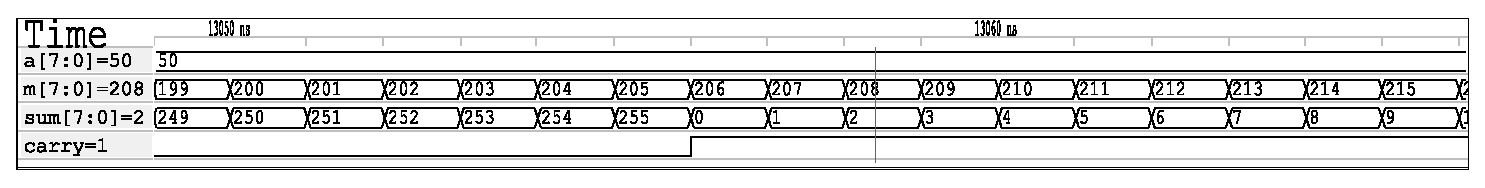
\includegraphics[scale=0.65]{../out/adder_tb.eps}
    \caption{Output waveform of the adder testbench from \SI{13049}{\nano\second} to \SI{13066}{\nano\second}.}
    \label{fig:addertbw}
\end{figure}

Figure \ref{fig:addertbw} shows a small section of the output waveform of the adder testbench. At the cursor's position, the values being added together are 50 and 208. In unsigned 8 bit binary, these are expressed as 0011 0010 and 1101 0000 respectively. Adding these two binary values together gives an answer of 1 0000 0010, or in decimal, 2 with a carry of 1, which corresponds to the shown waveform.

\section{Register design, simulation and synthesis}
An \lstinline{n} bit shift and add multiplier makes use of two \lstinline{n} bit registers, and a carry register. For no reason in particular, all three registers were combined in to one large register in this design. The \lstinline{RESET} instruction is invoked when the multiplier is in its idle state, i.e. waiting to start the calculation. It loads the multiplier in to the bottom 8 bits of the register. \lstinline{ADD} loads the results from the adder in to the top 8 bits of the register. The \lstinline{SHIFT} instruction right shifts the register by one position. \lstinline{SHIFT} and \lstinline{ADD} together carry out both instructions in one go.

\lstset{caption={Register code (regs.sv)}, label=ls:regs}
\begin{lstlisting}
`timescale 1ns/1ps
module regs(input logic clk, 
            input logic n_reset,
            input logic ADD,
            input logic SHIFT,
            input logic RESET,
            input logic[7:0] sum,
            input logic[7:0] multiplier,
            input logic carry,
            output logic[16:0] register);

    always @(posedge clk, negedge n_reset) begin
        if (!n_reset) begin
            register <= 0;
        end
        
        else if (RESET) begin
            register <= {9'b0, multiplier};
        end
            
        else if (ADD & !SHIFT) begin
            register[16:8] <= {carry, sum};
        end
            
        else if (SHIFT & !ADD) begin
            register <= {1'b0, register[16:1]};
        end
		
        // Implemented for carrying out the SHIFT and ADD in the same clock cycle.
        else if (SHIFT & ADD) begin
            register <= {1'b0, carry, sum, register[7:1]};
        end
        
        else begin
            register <= register;
        end
    end
endmodule
\end{lstlisting}

\subsection{Simulation of registers}
\lstset{caption={Register testbench (regs\_tb.sv)}, label=ls:regstb}
\begin{lstlisting}
`timescale 1ns/1ps
module regs_tb;
    logic clk;
    logic n_reset;
    logic ADD;
    logic SHIFT;
    logic[7:0] sum;
    logic[7:0] multiplier;
    logic carry;
    logic[16:0] register;
    logic RESET;
    
    int sumloop;
    int multiplierloop;
    int carryloop;
    
    regs r(.*);
    
    initial
    begin
        $dumpfile("regs_tb.vcd");
        $dumpvars(0, clk, n_reset, ADD, SHIFT, sum, multiplier, carry, register, RESET);
    end
    
    initial
    begin
        clk <= 0;
        forever #5 clk <= ~clk;
    end
    
    initial
    begin
        n_reset = 0;
        ADD = 0;
        SHIFT = 0;
        sum = 0;
        multiplier = 0;
        carry = 0;
        RESET = 0;
        
        #10;
        if (register != 9'b0)
        begin
            $display("Register isn't empty");
            $fatal;
        end
        
        // Some arbitrary values
        sum = 152;
        multiplier = 73;
        carry = 1;
        n_reset = 0;
        
        #10;
        n_reset = 1;
        RESET = 1;
        
        #10;
        if (register != 17'b00000000001001001)
        begin
            $display("Multiplier not loaded to register");
            $display("multiplier = %b, register = %b", multiplier, register);
            $fatal;
        end
        RESET = 0;
        ADD = 1;
        
        #10;
        if (register != 17'b11001100001001001)
        begin
            $display("Result from adder not loaded to register");
            $fatal;
        end
        ADD = 0;
        SHIFT = 1;
        
        #10;
        if (register != 17'b01100110000100100)
        begin
            $display("Register not shifted");
            $display("register = %b", register);
            $fatal;
        end
        SHIFT = 0;
        
        #10;
        if (register != 17'b01100110000100100)
        begin
            $display("Register not held");
            $display("register = %b", register);
            $fatal;
        end
        ADD = 1;
        SHIFT = 1;
        
        #10;
        if (register != 17'b01100110000010010)
        begin
            $display("Register not shiftadded");
            $display("register = %b", register);
            $fatal;
        end
        SHIFT = 0;
        ADD = 0;
        
        #10;
        RESET = 1;
        
        #10;
        if (register != 17'b00000000001001001)
        begin
            $display("Register not reset");
            $display("register = %b", register);
            $fatal;
        end
        
        #10;
        $display("Test passed!");
        $finish;
    end
endmodule
\end{lstlisting}

\begin{figure}[H]
    \centering
        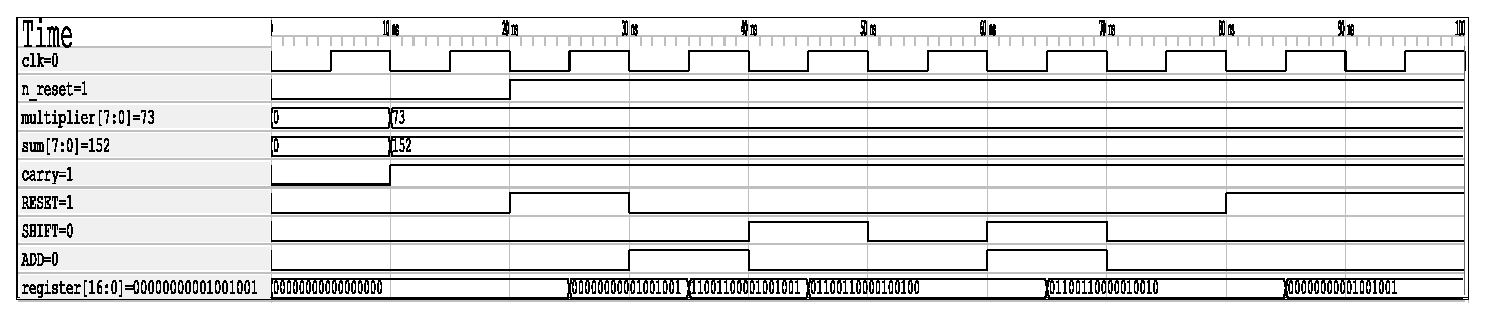
\includegraphics[scale=0.65]{../out/regs_tb.eps}
    \caption{Output waveform of the register testbench.}
    \label{fig:regstbw}
\end{figure}

The testbench for the register module as shown in listing \ref{ls:regstb} tests the register by checking its output value based on its operations on some arbitrary input values. After each stage it checks the value of the register to make sure that it is equal to the expected value.

Figure \ref{fig:regstbw} shows the resulting waveform of the testbench. As expected, despite being activated earlier, instructions are only executed on rising clock edges. This is shown as a change in the value of \lstinline{register[16:0]} in sync with a rising edge of \lstinline{clk}. For example, the multiplier is first loaded in to the register at \SI{25}{\nano\second}, at the same time as the clock edge. The changes in the register value are the same as those checked for in the testbench, showing that the register is working as expected.

\section{Sequencer design, simulation and synthesis}

The sequencer is the module that controls the entire operation, and implements the shift and add multiplication algorithm.

Figure \ref{fig:fseqASM} shows the ASM chart of final version of the state machine. It contains three distinct states, \lstinline{START}; \lstinline{DECREMENT, SHIFT}; and \lstinline{READY}, which are implemented in the module code as \lstinline{stIdle}; \lstinline{stAdd}; and \lstinline{stStop} respectively.

\begin{figure}[H]
    \centering
        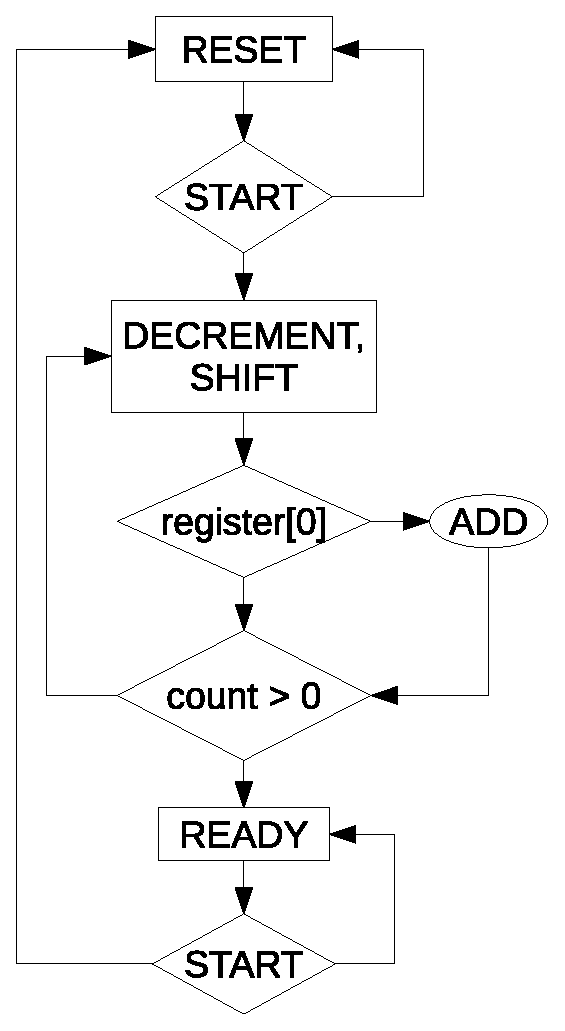
\includegraphics[scale=0.65]{finalSequencerASM.eps}
    \caption{ASM chart of the sequencer used in the final multiplier design.}
    \label{fig:fseqASM}
\end{figure}

\lstset{caption={Sequencer module (sequencer.sv)}, label=ls:seq}
\begin{lstlisting}
module sequencer(   input logic clk,
                    input logic[16:0] register,
                    input logic n_reset,
                    input logic START,
                    input logic[3:0] count,
                    output logic ADD,
                    output logic SHIFT,
                    output logic RESET,
                    output logic DECREMENT,
                    output logic READY);
                    
    typedef enum logic[2:0] {stIdle, stAdd, stShift, stStop} state;
    
    state stCurrent, stNext;
    
    initial
    begin
        $dumpfile("sequencer_tb.vcd");
        $dumpvars(0, stCurrent, stNext);
    end
    
    always @(posedge clk, negedge n_reset)
    begin
        if (!n_reset)
        begin
            stCurrent <= stIdle;
        end
        else
        begin
            stCurrent <= stNext;
        end
    end
    
    always @(*)
    begin
        #1ps;
        case (stCurrent)
            stIdle: begin
                RESET = 1;
                SHIFT = 0;
                ADD = 0;
                DECREMENT = 0;
                READY = 0;
                if (START) begin
                    stNext = stIdle;
                end
                else begin
                    stNext = stAdd;
                end
            end
            
            stAdd: begin
                RESET = 0;
                SHIFT = 1;
                DECREMENT = 1;
                READY = 0;
                if (register[0]) begin
                    ADD = 1;
                end
                else begin
                    ADD = 0;
                end
                if (count > 0) begin
                    stNext = stAdd;
                end
                else begin
                    stNext = stStop;
                end
            end
            
            stStop: begin
                RESET = 0;
                SHIFT = 0;
                DECREMENT = 0;
                ADD = 0;
                READY = 1;
                if (!START) begin
                    stNext = stIdle;
                end
                else begin
                    stNext = stStop;
                end
            end
            
            default: begin
                RESET = 0;
                SHIFT = 0;
                ADD = 0;
                DECREMENT = 0;
                READY = 0;
                stNext = stIdle;
            end
        endcase
    end
endmodule
\end{lstlisting}

\begin{figure}
    \centering
        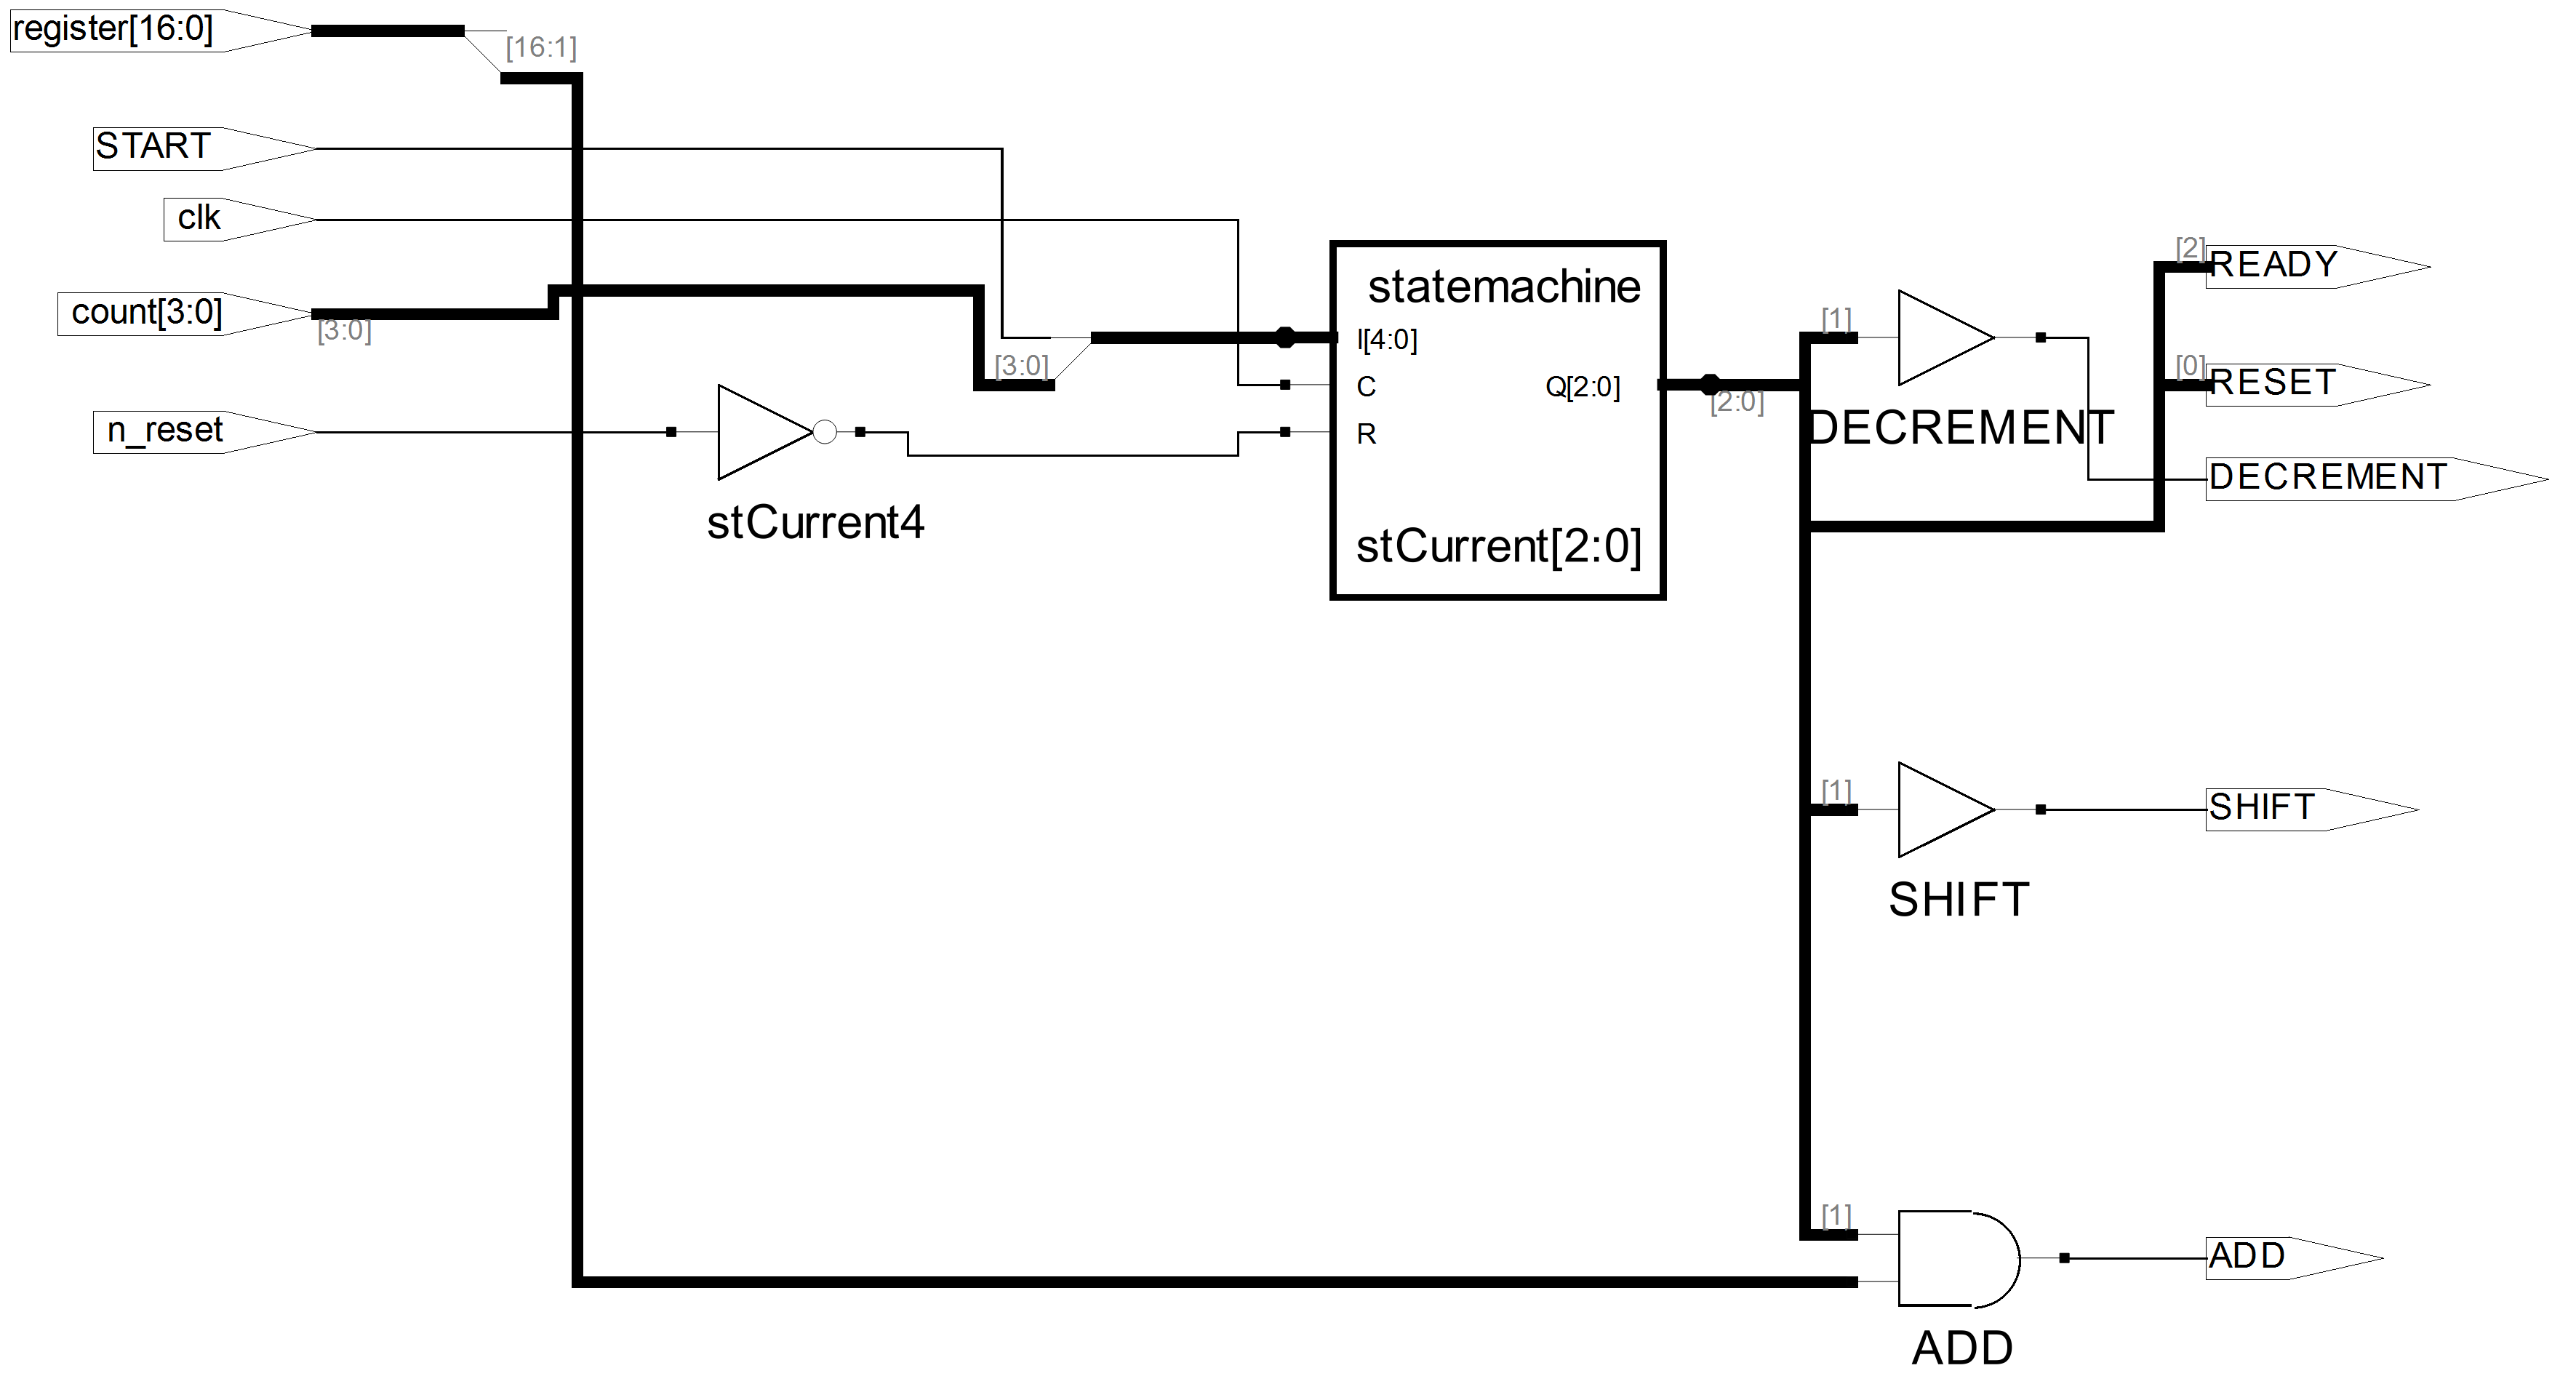
\includegraphics[scale=0.17]{./RTL/sequencer_c.png}
    \caption{RTL diagram of the sequencer module from Synpliy Pro}
    \label{fig:seqRTL}
\end{figure}

Upon starting the module, or invoking an asynchronous reset (\lstinline{n_reset = 0}), the sequencer should enter the \lstinline{RESET} or \lstinline{stIdle} state, where it instructs the register module to load the multiplier in to its lower 8 bits, and fill the rest with zeros. Whilst in this state, the sequencer also waits for a low \lstinline{START} signal, at which point the state machine will be instructed to go to to the \lstinline{stAdd} state. The code was initially written with the assumption that the button on the FPGA would be an active high input, hence the slightly counter-intuitive name of \lstinline{START}. Once in \lstinline{stAdd}, the \lstinline{DECREMENT} and \lstinline{SHIFT} signals are asserted, instructing the register to carry out a shift instruction, whilst decreasing the value of \lstinline{count} by 1. If the least significant bit of the register (or $Q_0$), the asynchronous output \lstinline{ADD} is asserted, which instead instructs the register to carry out a shift and add operation in one clock cycle. The sequencer then stays in the \lstinline{stAdd} state until it runs out of bits to work on, i.e. \lstinline{count = 0}, at which point the next state is asserted as \lstinline{stStop}. In \lstinline{stStop}, the sequencer asserts a \lstinline{READY} signal, telling the user that the calculation is complete. It also holds the value of the register, which is output to the user using a line of LEDs. The sequencer waits in this state until the \lstinline{START} signal goes low again. The \lstinline{count} variable is the output of a counter that starts at 7 and reduces by 1 every time the \lstinline{DECREMENT} signal is asserted.

\lstset{caption={Sequencer testbench (sequencer\_tb.sv)}, label=ls:seqtb}
\begin{lstlisting}
`timescale 1ns/1ps

module sequencer_tb;

    logic clk;
    logic[16:0] register;
    logic n_reset;
    logic START;
    logic[3:0] count;
    logic ADD;
    logic SHIFT;
    logic RESET;
    logic DECREMENT;
    logic READY;
    
    sequencer r(.*);
    
    initial
    begin
        $dumpfile("sequencer_tb.vcd");
        $dumpvars(0, clk, register, n_reset, START, count, ADD, SHIFT, RESET, DECREMENT, READY);
    end
    
    initial
    begin
        #5 clk = 0;
        forever #5 clk = ~clk;
    end
    
    initial
    begin
        register = 17'b000000000;
        n_reset = 0;
        START = 1;
        count = 4;
        
        #5;
        n_reset = 1;
        
        #5; // Should be in stIdle state
        if (ADD | SHIFT | !RESET | DECREMENT | READY) begin
            $display("Bad assertions!");
            $error;
        end
        
        #10; // Should still be in stIdle
        if (ADD | SHIFT | !RESET | DECREMENT | READY) begin
            $display("Bad assertions!");
            $error;
        end
        START = 0;
        
        #12; // Should be in stAdd. Not adding, since Q0 is 0.
        if (ADD | !SHIFT | RESET | !DECREMENT | READY) begin
            $display("Bad assertions!");
            $error;
        end
        START = 1;
        
        #10; // Should be in stAdd. Not adding, since Q0 is 0.
        if (ADD | !SHIFT | RESET | !DECREMENT | READY) begin
            $display("Bad assertions!");
            $error;
        end
        START = 0;
        register[0] = 1;
        
        #10; // Should be adding this time, since Q0 was 1.
        if (!ADD | !SHIFT | RESET | !DECREMENT | READY) begin
            $display("Bad assertions!");
            $error;
        end
        register[0] = 0;
        START = 1;
        
        #10; // Not adding, Q0 is 0 again.
        if (ADD | !SHIFT | RESET | !DECREMENT | READY) begin
            $display("Bad assertions!");
            $error;
        end
        count = 0;
        
        #10; // Should be finished here (stStop), since count = 0.
        if (ADD | SHIFT | RESET | DECREMENT | !READY) begin
            $display("Bad assertions!");
            $error;
        end
        START = 0;
        
        #10; // Should be back to stIdle.
        if (ADD | SHIFT | !RESET | DECREMENT | READY) begin
            $display("Bad assertions!");
            $error;
        end
        
        $finish;
    end
endmodule
\end{lstlisting}

\begin{figure}[H]
    \centering
        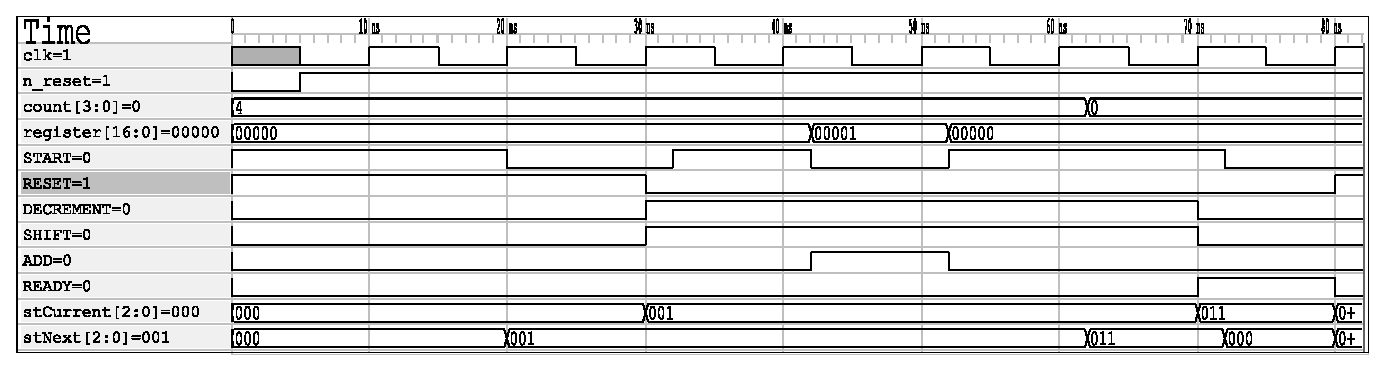
\includegraphics[scale=0.65]{../out/sequencer_tb.eps}
    \caption{Output waveform of the sequencer testbench.}
    \label{fig:seqtbw}
\end{figure}

The testbench of the sequencer (listing \ref{ls:seqtb}) goes through each state of the sequencer and makes sure that the appropriate output signals are asserted. It does this by modifying the input signals and checking to see that the sequencer goes in to the correct state by checking the output signals. Input signals are also modified such that the conditional outputs get asserted, for example, by setting \lstinline{register[0] = 1} in line 66, in which case the ADD output signal should be asserted. The \lstinline{START} signal gets toggled at some points throughout the test to make sure that the sequencer does not react to it unless it's in the \lstinline{stIdle} or \lstinline{stStop} state. Figure \ref{fig:seqtbw} shows how the state machine reacts to various inputs, and also shows the states of the machine. Here, state 000 is \lstinline{stIdle}, state 001 is \lstinline{stAdd}, and state 011 is \lstinline{stStop}. State 010 is not shown, since it was not used in the final code.

\section{Multiplier design, simulation and synthesis}

The final required module is the multiplier itself. Its job is to actually wire all the other modules together, and to provide the clock signal for the register and sequencer.

\lstset{caption={Multiplier module (multiplier.sv)}, label=ls:mul}
\begin{lstlisting}
`timescale 1ns/1ps
module multiplier(  input logic START,
                    input logic n_reset,
                    output logic[15:0] AQ,
                    output logic READY);
                    
    logic hwClock;
    logic clk;
    logic carry;
    logic RESET;
    logic SHIFT;
    logic ADD;
    logic DECREMENT;
    logic[7:0] multiplicand;
    logic[7:0] multiplier;
    logic[7:0] sum;
    logic[16:0] register;
    logic[3:0] count;
    
    initial
    begin
        $dumpfile("multiplier_tb.vcd");
        $dumpvars(0, hwClock, clk, carry, RESET, SHIFT, ADD, DECREMENT, multiplicand, multiplier, sum, register, count);
    end
    
    //Comment out if synthesising!
    // initial
    // begin
        // clk = 0;
        // forever #1 clk = ~clk;
    // end
    
    // For conformance with specification
    assign AQ = register[15:0];
    
    //// Internal Oscillator 3.33MHz. Comment out if simulating!
    defparam OSCH_inst.NOM_FREQ = "3.33";
    OSCH OSCH_inst
        ( 
        .STDBY(1'b0),       // 0=Enabled, 1=Disabled also Disabled with Bandgap=OFF
        .OSC(hwClock),
        .SEDSTDBY()             // this signal is not required if not using SED
        );
        
    assign multiplicand = 8'b11001011;
    assign multiplier = 8'b00010011;
    
    slowClock sc(.*);
    adder a(.a(register[15:8]), .m(multiplicand), .carry(carry), .sum(sum));
    regs r(.*);
    counter c(.*);
    sequencer s(.*);
    
endmodule

\end{lstlisting}

\begin{figure}[H]
    \centering
        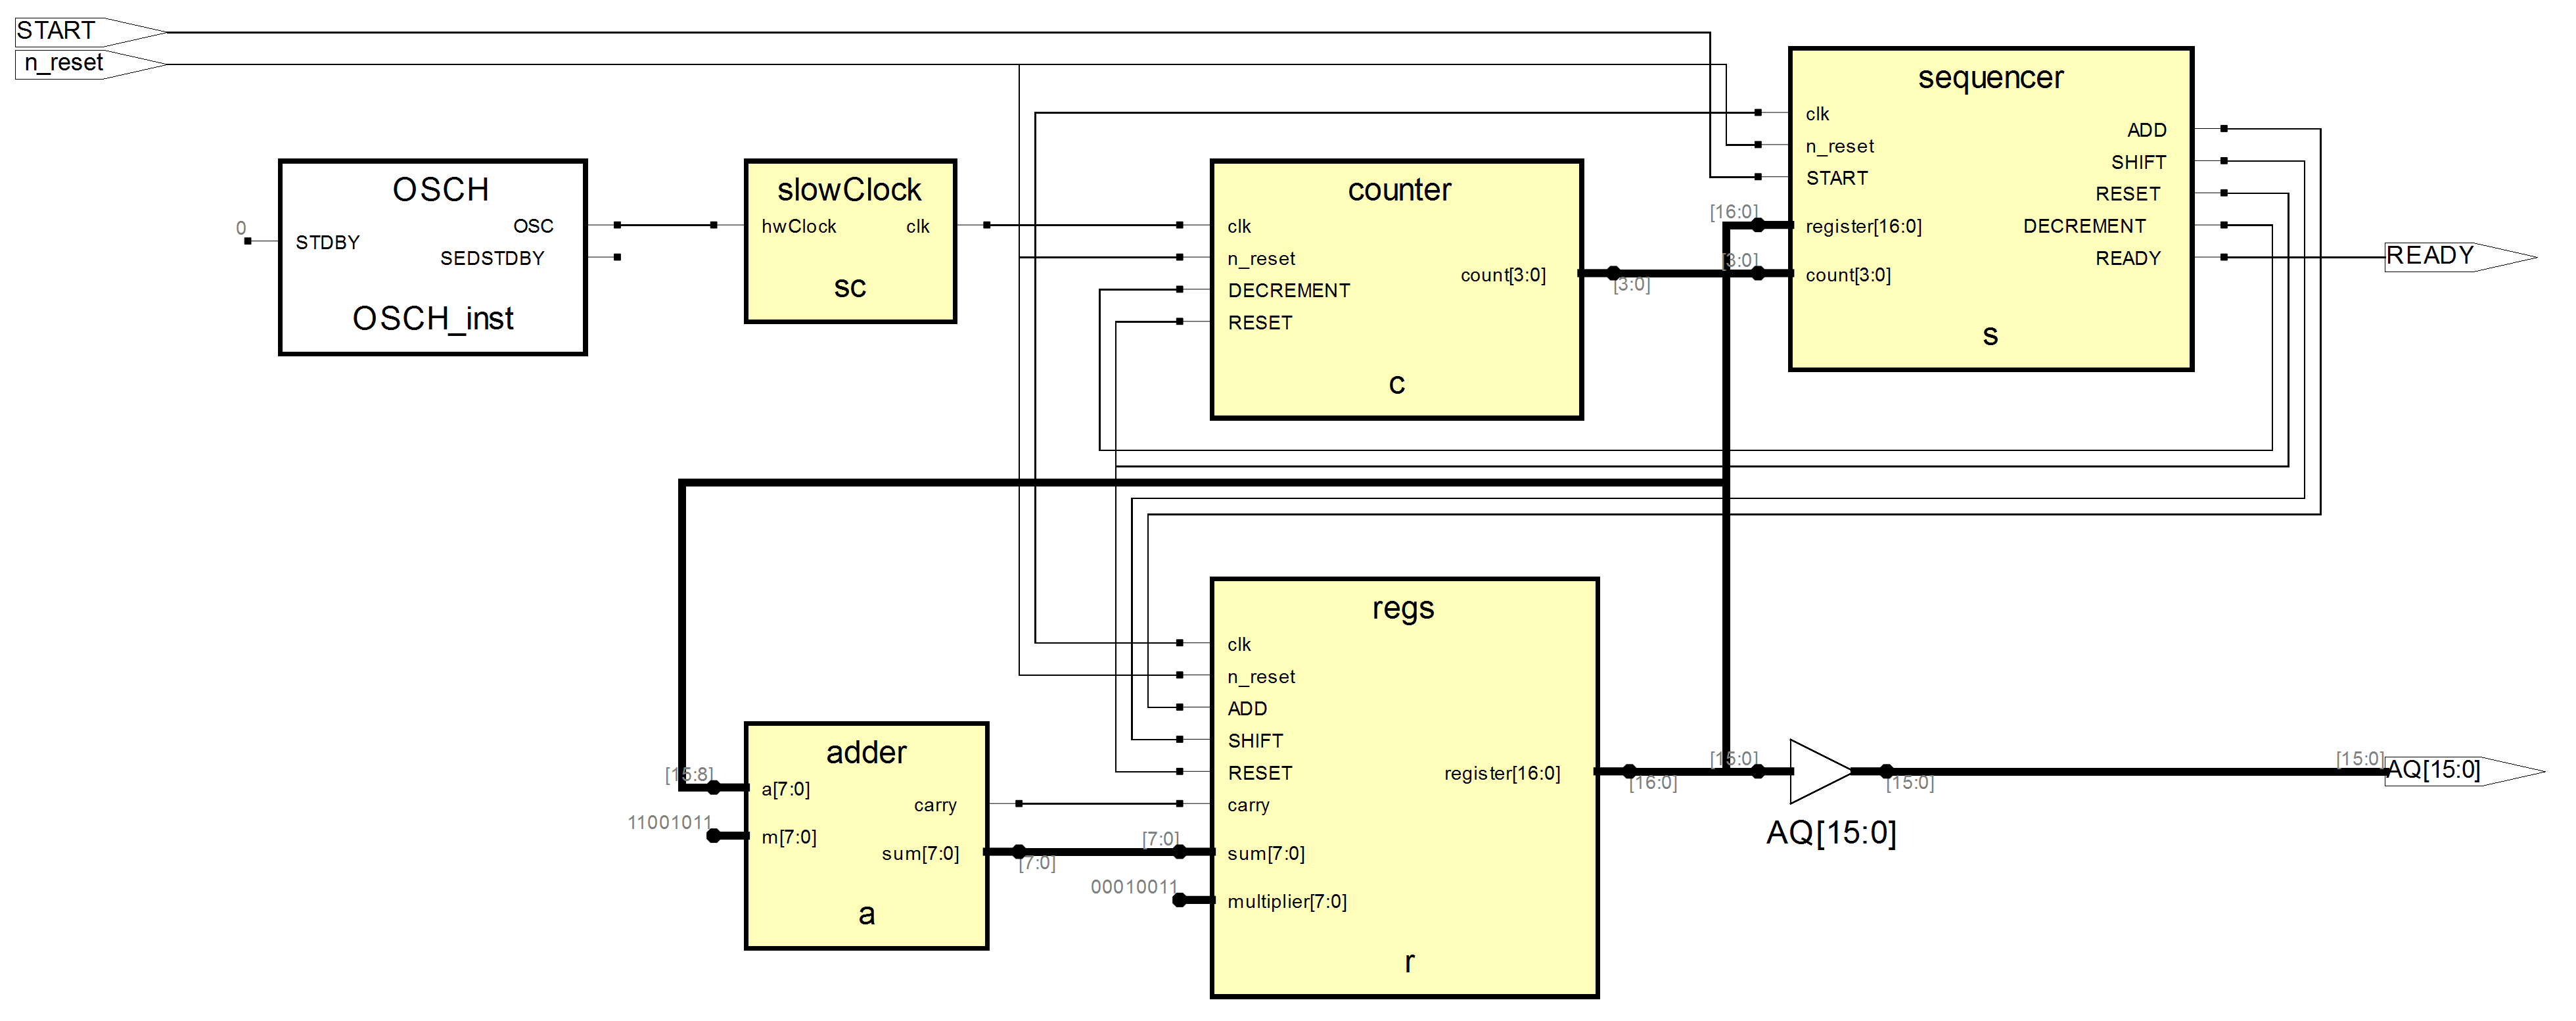
\includegraphics[scale=0.15]{./RTL/multiplier_c.png}
    \caption{RTL diagram of the multiplier module from Synpliy Pro}
    \label{fig:mulRTL}
\end{figure}

The code in listing \ref{ls:mul} is fundamentally unchanged from the model code provided~\cite{multipliercode}, except for some naming changes. \lstinline{M} and \lstinline{Q} were changed to \lstinline{multiplicand} and \lstinline{multiplier} respectively to prevent confusion. The specification required the working values in the ``AQ'' register to be shown. Since in this case, the registers were implemented as a single large register, with C, A and Q all in one, the \lstinline{AQ} assignment was added in line 34.

The \lstinline{slowClock} module is identical to the model one provided~\cite{slockcode}, except with some variables renamed again. Its job is to divide the FPGA's internal \SI{3.33}{\mega\hertz} clock down to a more managable rate, so that the calculation steps of the multiplier are actually visible to humans. Although, when simulating, the hardware clock was not used. Instead, the block starting at line 27 was used to generate the clock signal, and the instance of \lstinline{slowClock} was commented out. This is because the simulator doesn't understand what to do with a hardware clock, and since the simulation will not be analised in realtime anyway, the slow clock generator is not necessary.

\lstset{caption={Multiplier testbench (multiplier\_tb.sv)}, label=ls:multb}
\begin{lstlisting}
`timescale 1ns/1ps

module multiplier_tb;
    
    logic START;
    logic READY;
    logic n_reset;
    logic[15:0] AQ;
    
    multiplier m(.*);
    
    initial
    begin
        $dumpfile("multiplier_tb.vcd");
        $dumpvars(0, AQ, n_reset, START, READY);
    end
    
    initial
    begin
        n_reset = 1;
        START = 0;
        
        #500ps
        n_reset = 0;
        #100ps
        n_reset = 1;
        
        #2400ps;
        n_reset = 1;
        
        #1;
        START = 1;

        #2;
        START = 0;
        
        #29
        START = 1;

        #6;
        START = 0;
        
        #30;
        n_reset = 0;
        
        #5;
        $finish;
    end
endmodule
\end{lstlisting}

\begin{figure}[H]
    \centering
        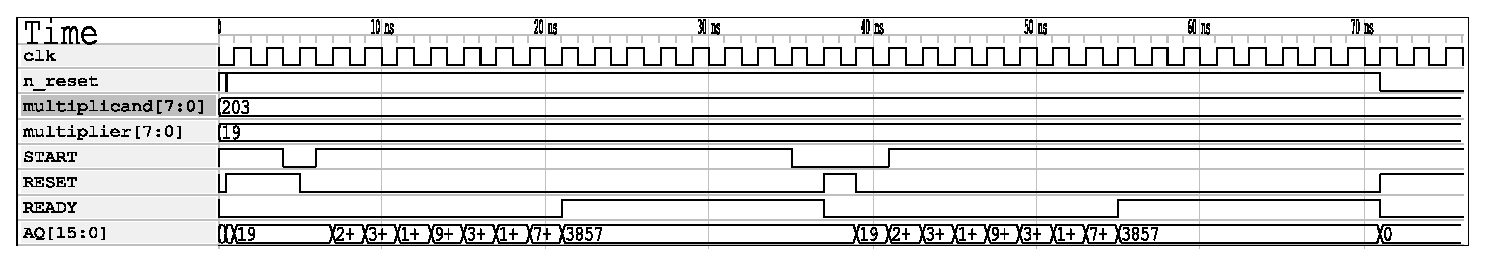
\includegraphics[scale=0.65]{../out/multiplier_tb.eps}
    \caption{Output waveform of the multiplier testbench.}
    \label{fig:multbw}
\end{figure}

The multiplier testbench (listing \ref{ls:multb}) simply simulates the end user operation of the device. It is initially reset, and then the START signal is set low to start the calculation. As shown in listing \ref{ls:mul} and figure \ref{fig:multbw}, the input being tested is $203\times19$. The \lstinline{AQ} register is visible at at the bottom of the waveform, and shows that when the multiplier is done (\lstinline{READY} is high), the answer is $3857$, which is correct. The sequence gets tested again to make sure that the multiplier goes back to the beginning, ready to calculate again.

\section{Extensions}

The main task was to design a 4 bit multiplier that followed the algorithm outlined in the D1 brief. Two extension tasks were carried out. The first being the implementation of the \lstinline{SHIFT} and \lstinline{ADD} instructions being combined in to the same clock cycle. This involved creating the insturction on line 31 of listing \ref{ls:regs} for the register to carry out when both \lstinline{SHIFT} and \lstinline{ADD} signals were asserted. The sequencer then had to be modified to combine \lstinline{stAdd} and \lstinline{stShift} (from listing \ref{ls:stShift}) in to one state. Since \lstinline{SHIFT} and \lstinline{DECREMENT} would be asserted every single time before checking the value of $Q_0$, it meant that the check and \lstinline{SHIFT} assertion could be easily moved to the \lstinline{stAdd} state.

\lstset{caption={Sequencer shift state}, label=ls:stShift}
\begin{lstlisting}
stShift: begin
    RESET = 0;
    SHIFT = 1;
    DECREMENT = 0;
    ADD = 0;
    READY = 0;
    if (register[0]) begin
        if (count > 0) begin
            ADD = 1;
            stNext = stAdd;
        end
        else begin
            ADD = 0;
            stNext = stStop;
        end
    end
    else begin
        ADD = 0;
        stNext = stAdd;
    end
end
\end{lstlisting}

Since this combines two of the main operations of the multiplier in to a single clock cycle, it noticably improves its speed at slow clocks.

The other extension was to implement an 8 bit multiplier instead of a 4 bit. This was rather trivial, since all that had to be done was to double the size of every register in the design, except for the 1 bit inputs/outputs, and the counter. After assigning all the extra bits of \lstinline{AQ} to extra output pins, the design worked as intended. It took roughly twice as long to complete a calculation.

\section{Conclusion}

An 8 bit multiplier using the shift and add algorithm with the \lstinline{SHIFT} and \lstinline{ADD} instructions combined in to a single clock cycle has been implemented for the MachXO2 Pico FPGA.

One of the things I learnt during this design exercise, while likely only applicable to my SystemVerilog environment (Icarus Verilog), is to make sure that delays are specified in the correct part of a line. \lstinline{#1 forever clk = ~clk;} would cause the simulation to hang and leak memory until it was stopped, or the system crashed. I think that because there are no delays within the loop itself, the simulator was trying to do an infinite number of \lstinline{clk} assignments at a single point in time. \lstinline{forever #1 clk = ~clk;} would produce the desired result.

The design could have been improved by parameterising the size of the multiplier. Instead of changing the size of every register manually when going from 4 to 8 bit, I could have written it so that all that was necessary was to change the value of a single variable from 4 to 8. Of course, it should work with any value, not just 4 and 8.

\section{References}
\bibliographystyle{IEEEtran}
% IEEEabrv abbreviates journal titles in accordance to IEEE standards 
\bibliography{IEEEabrv,mybib}
  
\end{document}